\documentclass[../Assignment-3-LPSMT.tex]{subfiles}
\graphicspath{{\subfix{../img/}}}

\begin{document}

\chapter{Implementazione}

Manga-check è stata sviluppata seguendo un modello a singola Activity con un
\href{https://developer.android.com/guide/navigation}{controller di navigazione}
che funge da istanziatore e sistema di passaggio di parametri da un fragment ad un altro.\\

\section{Divisione in moduli}

\section{Struttura del DB}

\lstinputlisting[language=Kotlin, caption={Parte di Series.kt}]{snippet-codice/Series.kt}

\lstinputlisting[language=Kotlin, caption={Parte di Chapter.kt}]{snippet-codice/Chapter.kt}

Nella definizione di Chapter abbiamo usato l'attributo \texttt{unique} per poter poi verificare la presenza di numeri duplicati e quindi fermare l'utente dall'inserimento.

\section{Richieste API}

Le richieste API sono state gestite con il sopracitato package \emph{Apollo}, per garantire una fruibilità maggiore tutte le richieste vengono gestite in un Thread separato rieptto a quello della UI.\\
Per ricevere i dati abbiamo usato dei \href{https://developer.android.com/reference/kotlin/androidx/lifecycle/LiveData}{LiveData}, quindi una volta che i dati sono effettivamente presenti vengono mostrati a UI, le immagini vengono gestite grazie a \emph{Glide}.\\
Le entry così generate vengono inserite in una RecyclerView con la quale l'utente andrà ad interagire.

\lstinputlisting[language=Kotlin, caption={Parte del codice usato per fare le Query}]{snippet-codice/Query.kt}

\section{Uso di Safe Args}

Nel progetto abbiamo dovuto trasferire alcuni dati tra due fragment, come indicato nella documentazione Android abbiamo deciso di usare il \emph{navigation graph}, quindi vincolando i dati ad avere un determinato tipo.\\
Questo vincolo è stato possibile grazie all'utilizzo del plug in \href{https://developer.android.com/guide/navigation/use-graph/pass-data#Safe-args}{Safe Args} che ci ha permesso di specificare delle \emph{action} con un paylod di dati tipizzati.\\

\begin{center}
  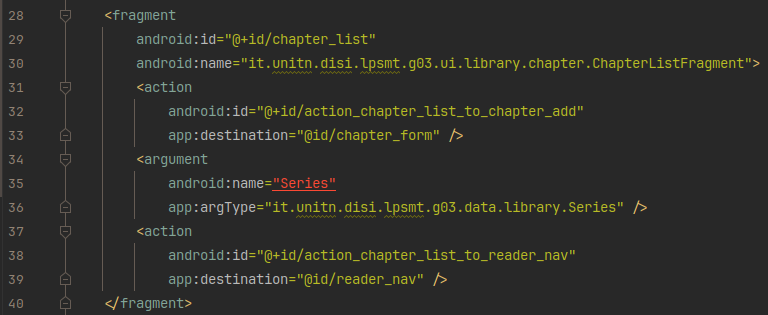
\includegraphics[scale=0.5]{action_navgraph.png}
  \captionof{figure}{Esempio di action con Safe Args}
\end{center}

\section{Backup Del DB}

Utilizzando le \href{https://developer.android.com/guide/topics/data/autobackup}{funzionalità native} di Android abbiamo implementato un sistema di Backup che permette all'utente di spostare la reading list senza bisogno di esportare alcun file.\\
Abbiamo usato le proprietà del manifest per indicare ad Android di effettuare il back-up dei file dell'applicazione e di permettere il trasferimento dei file quando si avvicina un nuovo dispositivo da inizializzare.

\section{Reader}

I \emph{cbz} vengono prima decompressi in cache, cosi da non occupare troppa RAM, una volta fatto ciò, i file vengono converti durante l'esecuzione in Bitmap ridimensionate per coprire più superficie possibile.\\
Successivamente le Bitmap vengono gestite sempre da \emph{Glide}, questo ci assicura un'esecuzione asincrona e minimizza il codice da sceivere.\\
Abbiamo anche implementato delle variabili per tenere conto della pagina alla quale è arrivato l'utente, queste variabili sono servite anche per la produzione della barra di progresso nella selezione dei capitoli.

\end{document}
